\section{Identification of the Cause of Drift}

At this point we think it necessary to perform a simple experiment in order to determine if the drift is being caused by the laser or by a crystal. We still somewhat believe the change to be temperature related, as few other measurements follow such clear stabilization curves as shown in \cref{fig:DE0} and \cref{fig:DE1}. This experiment works exactly as the previous two, however prior to running the test we will allow for the laser to warm up while being blocked for three hours. The results of this test are shown in \cref{fig:DE2}.

This test shows that the majority of the drift that we've seen in earlier experiments is in fact due to some effect of the laser. However, the experiment also shows that even once the laser is `stabilized' the percentage of $\HH$ detections can still move around on the order of 0.1\% every hour. This is bound to cause issues in our experiments, especially with the preset state calibrations, but we will just have to work around it for now.

\begin{figure}
	\centering
	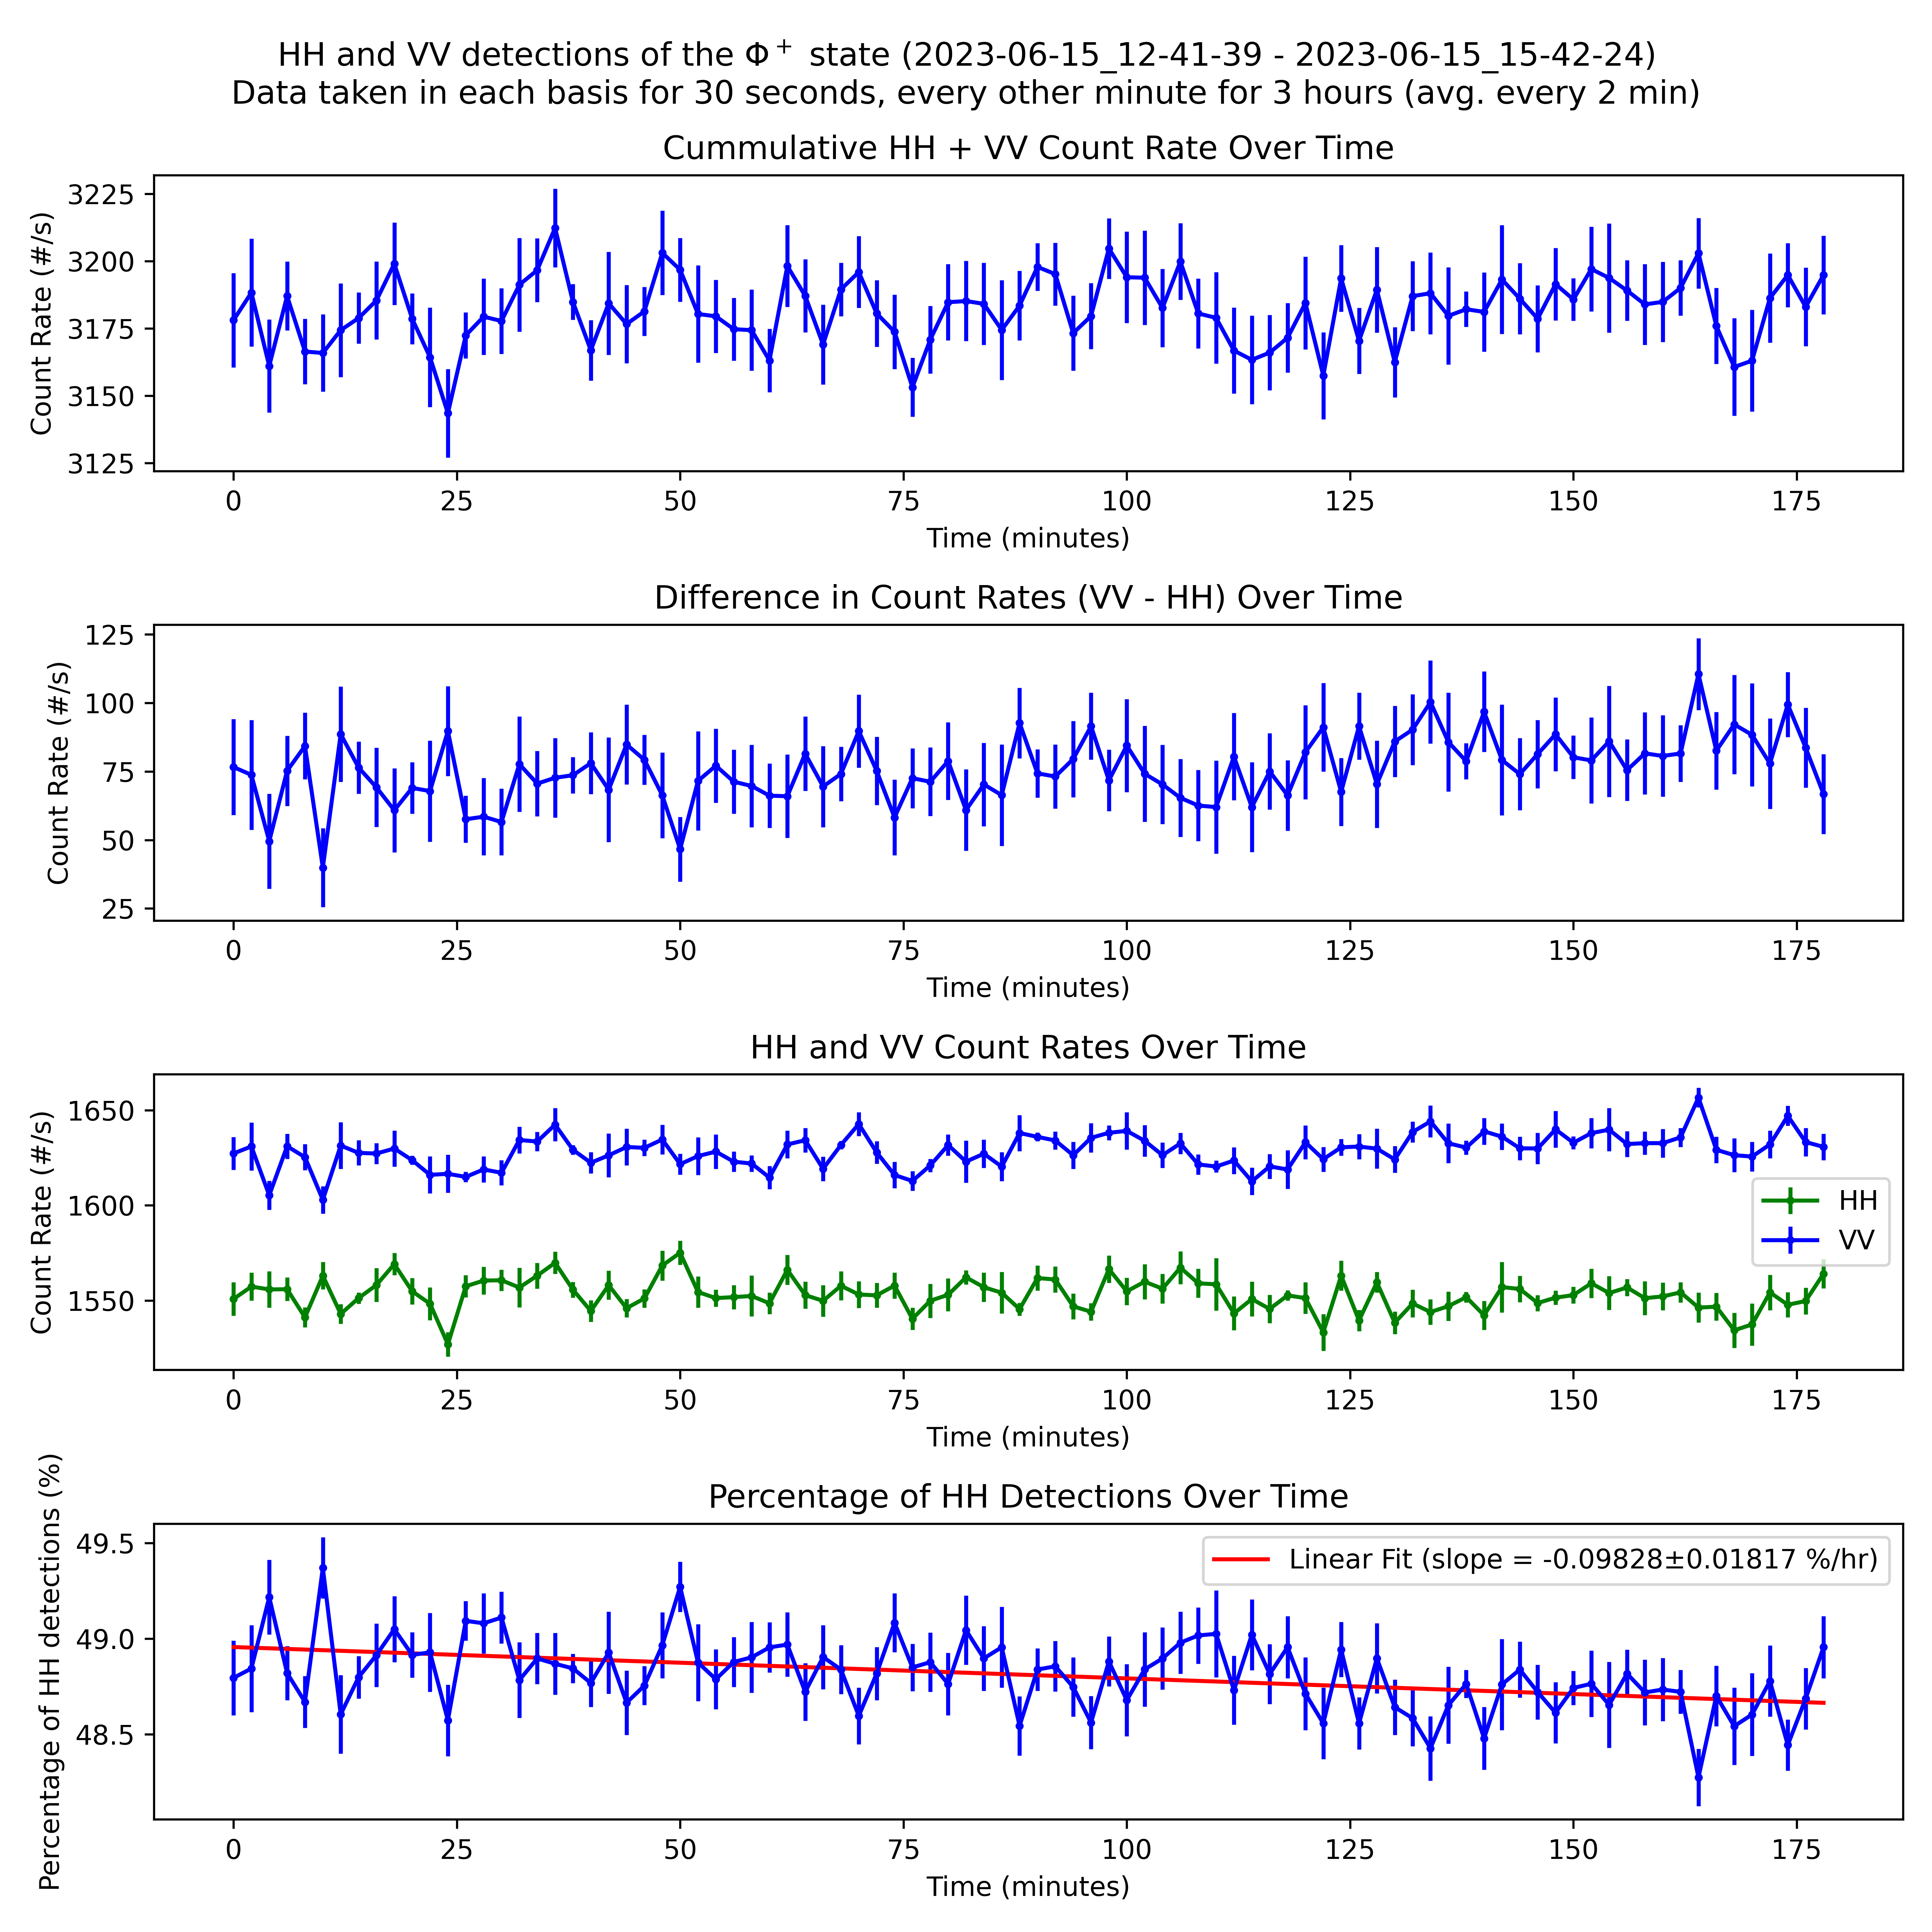
\includegraphics[width=\textwidth]{DE2_plot.png}	
	\caption{In this experiment, the laser was allowed to warm up for three hours prior to data collection. However, as you can see from the linear fit that is plotted, we still are seeing movement of the $\HH$ percentage count away from 50:50. This experiment was a bit discouraging, however when compared to \cref{fig:DE0} and \cref{fig:DE1} there is certainly a drastic difference in terms of the initial drift. The linear fit on this plot actually seems justified, whereas the others began with a clear and sharp drop.}
	\label{fig:DE2}
\end{figure}

We suspect that the laser drift is either due to or proportional to modulation laser's te






